\chapter{User's Documentation}

This section presents our game to the player and explains its installation, startup and controls. The playable version of our game
can be found on the attached DVD as Attachment~C.

\section{Installation and startup}

The game requires Windows~7 or a newer Windows operating system to run. Additionally, it requires a graphics card that is compatible
with either OpenGL~3 or Direct3D 9.

To install the game, we should first move the directory that contains the game's executable file anywhere on our hard disk. Although this is
an optional step, it allows our game to create new files which allows us to use the save feature of the game. Next, we need to install
the Visual C++ Redistributable, which can be done by executing the file \texttt{deps/vc\_redist.x86.exe}.

Once the redistributable is installed, we can start the game by executing the file \texttt{tdt.exe}. If this is the first startup, we will
see a window that allows us to configure our graphics options, which can be seen in Figure~\ref{ogre-config}. In this window, we need to
choose either the OpenGL or Direct3D from a drop-down list labeled \emph{Rendering Subsystem}. Once we choose our rendering subsystem, we
will be offered with various graphical settings we can change in the bottom list labaled \emph{Rendering System Options}. We will now also
be able to start the game by clicking on the \emph{OK} button.

\begin{figure}[H]
    \centering
    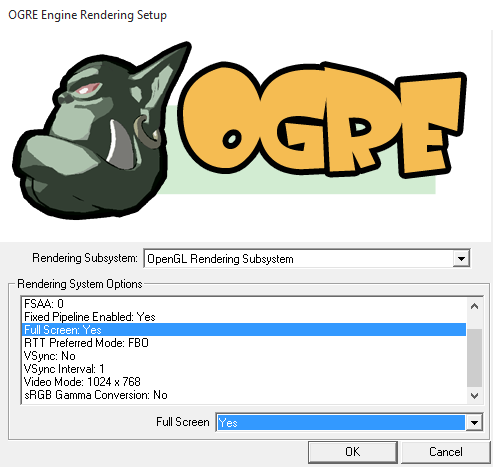
\includegraphics[width=10cm]{../img/ogre-cfg.png}
    \caption{Initial graphics setting window that is shown on the first start of the game.}
    \label{ogre-config}
\end{figure}

Next time we start the game, this window will not appear and the game will use the settings we chose the first time. If we want to change
these settings, we can force this window to appear on the next start of the game by deleting the file \texttt{ogre.conf}.

\section{Main menu}

\begin{figure}[H]
    \centering
    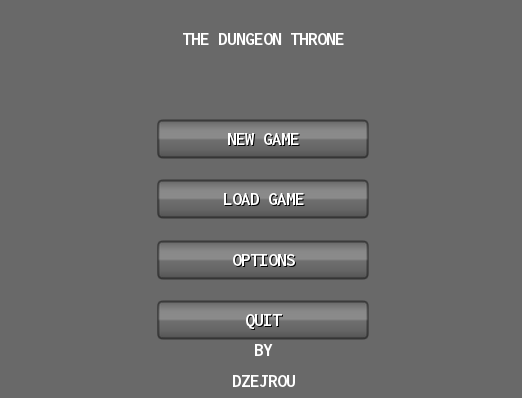
\includegraphics[width=10cm]{../img/gui-intro.png}
    \caption{Initial menu that we can see when we start the game.}
    \label{gui-intro}
\end{figure}

When the game starts, we will be greeted by the game's main menu, which can be seen in Figure~\ref{gui-intro}. In this menu, we can create
a new game by clicking on the button \emph{NEW GAME}, which shows a window that will prompt us for level dimensions. Here, we can either
input any pair of numbers in the given range, or choose one of the buttons with predefined dimensions.

If we already have a previously saved game, we can click the button \emph{LOAD GAME}, which will show a window all saved games that are
located in the \texttt{saves} directory. Aside from starting a level -- be it a new one or a loaded one -- we can view the options menu by
clicking on the button labeled \emph{OPTIONS} or close the game with the \emph{QUIT} button.

\section{User interface}

When we get into the game, we have a similar view to the one shown in Figure~\ref{gui-full}. At the top of the screen, we can see the top
bar, which displays our current resources -- our gold, our current and maximum mana with mana regeneration in parentheses, current number
of minions we control and the total number of minions we have, which includes minions that died and are respawning. Next to these resources,
we can also see the current system time.

Below the top bar, we can see the game world. The game world consists of blocks, which represent walls and buildings, our minions and
attacking enemies. In the image we can see a starting area of a newly generated world, which includes a free area in the middle where
the player's dungeon throne -- which represents the life of the player -- is placed along with some other starting building. We can select
any entity by either clicking on it with our left mouse button or by pressing the mouse button and dragging the mouse which allows us
to select multiple entities.

At the bottom of the screen, we can see three large windows. The one of the left is the tool bar. This window can contain three different
tool bars that can be switched between by clicking on one of the buttons located in the top row of the tool bar. The menu shown by default
is used to save and load the game and to show the options, main menu and research window. If we click on the \emph{SPELL} button the tool bar
changes to the spell bar, which can be used to cast spells, and if we click on the \emph{BUILD} button the tool bar changes to the building
bar, which can be used to place new buildings. The last button on the top row, \emph{MENU}, returns us to the initial menu bar.

Next to the tool bar is the game log, which shows messages from the game and from the player's minions. These message can for example include
warnings about an attack or notifications about insufficient resources.

The rightmost of these three windows is the entity viewer, which shows information about the currently selected single entity -- note that
it will not show anything when we select multiple entities. This information includes data such as the health, mana, level and name of the
selected entity. Besides the information shown, the entity viewer contains two buttons. The left button can be used to convert gold to
experience, which can be used to quickly level the entity up, and the right button can be used to sacrifice our entity in return for a part
of its cost.

Above the entity viewer window, we can see a small countdown bar, which tells us the time before the next wave of enemies will attack our
dungeon.

\begin{figure}[H]
    \centering
    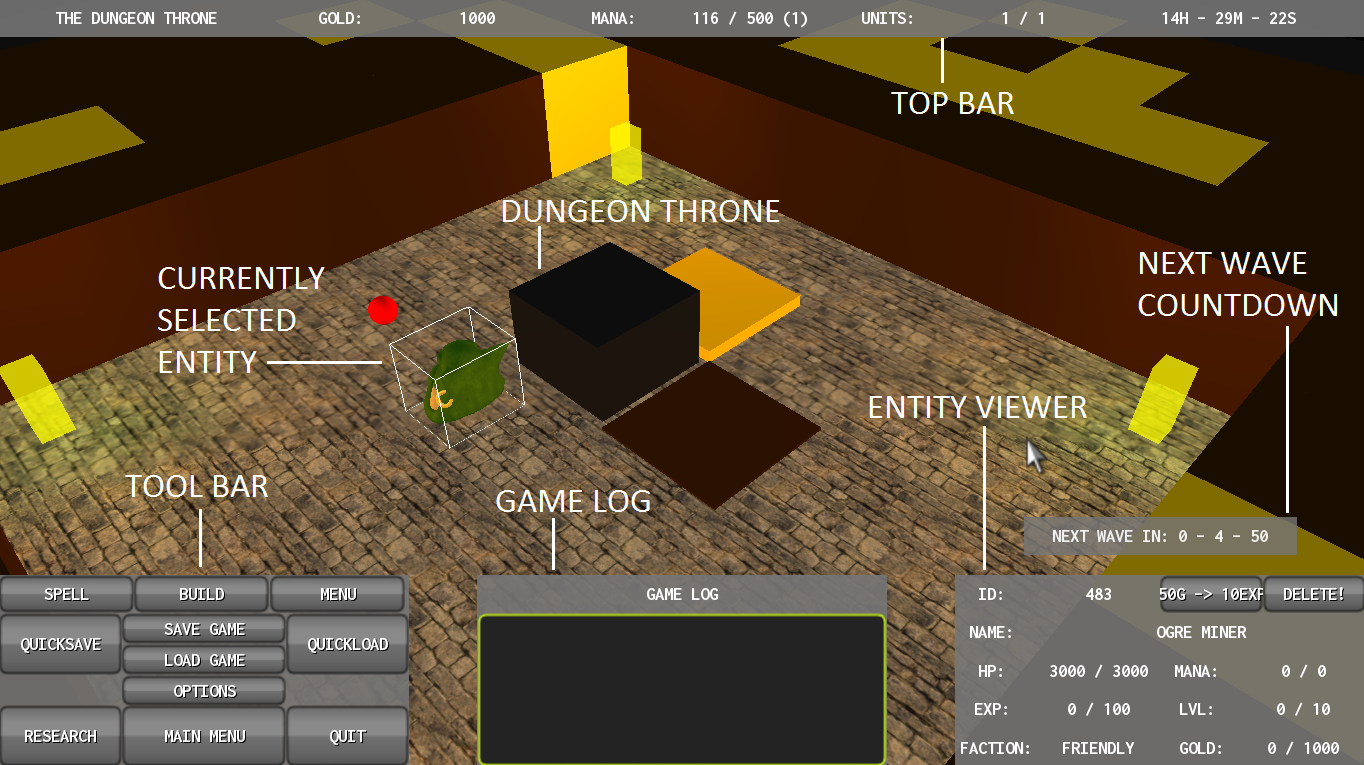
\includegraphics[width=\textwidth]{../img/gui-full-text.png}
    \caption{The game screen.}
    \label{gui-full}
\end{figure}

\section{Goal of the game}

In our game, the main goal of the player is to protect its dungeon -- specifically the dungeon throne -- from waves of enemy attackers
\footnote{Note that this applies to the game itself, mods are free to change the winning or losing conditions.}.
If the dungeon throne is destroyed, the player loses. If, on the other hand, the throne survives all of the enemy waves, the player wins.

To protect the dungeon throne, the player can place buildings in exchange for gold gathered by miners and cast spells that can damage or slow
the enemies in exchange for mana, which automatically regenerates. When a new level is created, the player starts with a small area that
contains the dungeon throne, a mine that spawns a miner and a gold vault that the miner uses for gold storage. Additionally, one side of a
map will contain enemy spawners, which will spawn enemies in intervals defined by the game's wave system.

Some of the buildings can spawn minions that will defend the dungeon from enemies and will revive these minions when and if they are killed.
To unlock these and other buildings, as well as new spells, the player can use the research window that is accessible from the menu tool
bar to exchange gold for new research unlocks that can provide buildings, spells or one time bonuses to the player.

Once all enemy waves are beaten, the player will be presented with the option to play in a sandbox mode, which allows them to continue
building their dungeon without any further enemy waves, or in an endless mode, which will repeat the last enemy wave indefinitely.

\section{Research}

Research is the tool we can use to unlock new buildings, spells and bonuses. The research window, which can be seen in
Figure~\ref{gui-research}, contains six rows that have seven tiers of unlock nodes each. To unlock a node, one can click on the research
button that represents it and, if they have enough gold, the unlock takes effect.

There are three types of unlocks in the game -- one time bonuses, building unlocks and spell unlocks. To avoid redundancy, we will
list one time bonuses with their effects here and the rest of the unlocks -- that is, buildings and spells -- will be described in the
following chapters.

\begin{itemize}
    \item \emph{KILL ALL ENEMIES} -- kills all enemy entities in the world.
    \item \emph{INCREASE PROD.} -- increases the production limit of all friendly buildings by one.
    \item \emph{DOUBLE PROD.} -- doubles the production limit of all friendly buildings by one.
    \item \emph{LEVEL UP} -- increases the level of all friendly entities.
    \item \emph{UBER THRONE} -- heals the dungeon throne and increases its health and defense.
    \item \emph{INSTANT PROD.} -- causes all buildings to spawn minions without waiting.
\end{itemize}

The research nodes have unified unlock cost per tier. The cost is 200, 400, 600, 800, 1000, 1500 and 2000 gold for tiers 1, 2, 3, 4, 5, 6 and
7 respectively. When a research node is unlocked, its name gets prefixed with a plus symbol and the next research node in the row is revealed.

\begin{figure}[H]
    \centering
    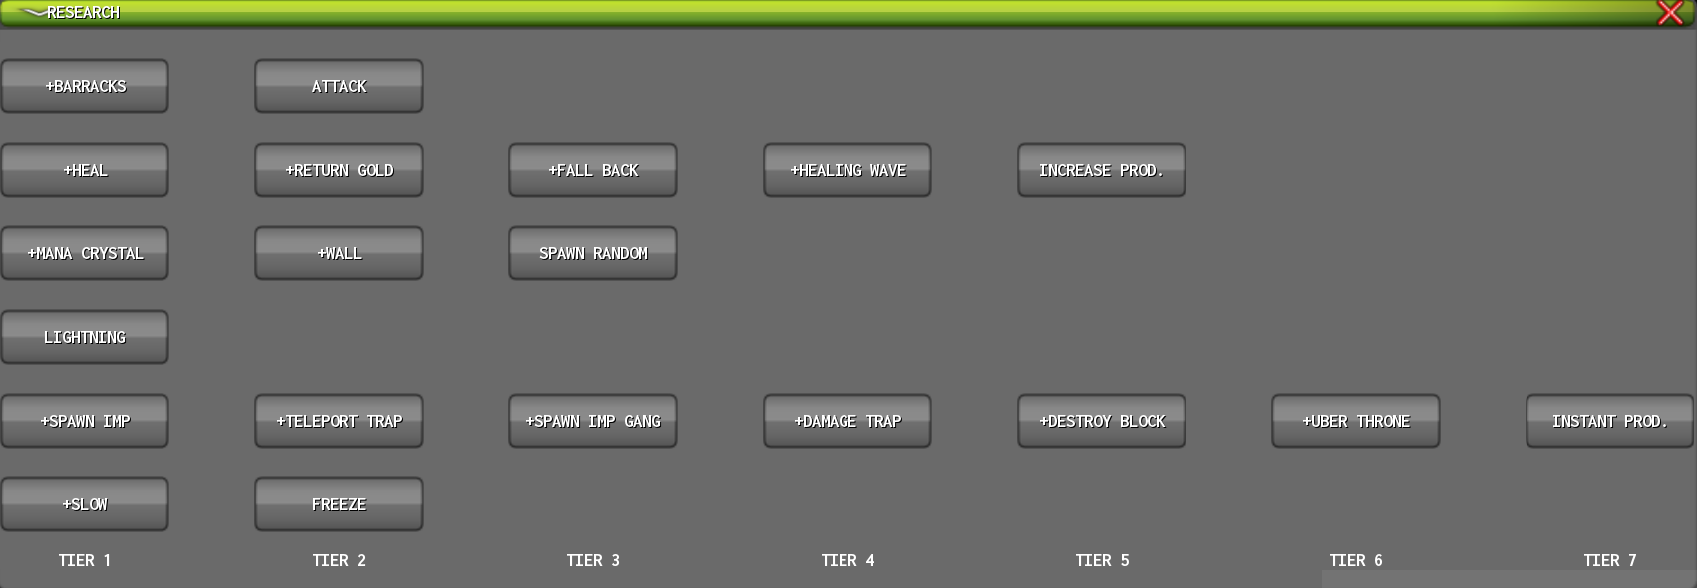
\includegraphics[width=\textwidth]{../img/gui-research.png}
    \caption{Research window which contains nodes that can be unlocked.}
    \label{gui-research}
\end{figure}

\section{Spell casting}

Spells are the means for the player to directly affect the battles between their minions and attacking enemies. Most spells are unlocked
through the research window\footnote{Those that are not are available to the player from the start of the game.}, in which a research
node \emph{SPELL NAME} unlocks spell \emph{spell\_name}.

We can cast spells through the spell tool bar window, which can be shown by clicking on the \emph{SPELL} button that is located in the
top row of buttons in the tool bar window. We can see a picture of the spell tool bar in Figure~\ref{gui-spell}. From top to bottom, it
contains a row of buttons that can be used to switch to other tool bars, a row of four buttons that represent different spells and two
buttons on the bottom row that are used to switch between spells.

\begin{figure}[H]
    \centering
    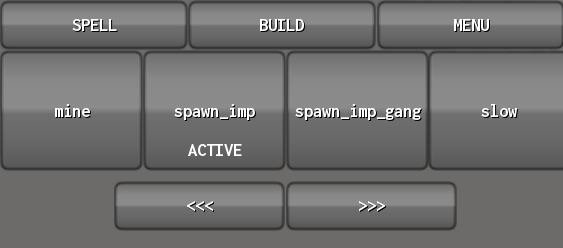
\includegraphics[width=\textwidth]{../img/tool-spell.png}
    \caption{Window that allows the player to cast spells.}
    \label{gui-spell}
\end{figure}

We can think of the spell tool bar as of a conveyor belt which contains our spells in the order we have unlocked them. The
\emph{\textless\textless\textless} button moves the belt to the left by one spell and the \emph{\textgreater\textgreater\textgreater}
button moves it to the right by one spell. Once we locate the spell we would
like to cast, we can either click on it with the left mouse button or press the key assigned to it -- these four spell buttons correspond
to key binding actions \emph{SPELL/BUILD 1-4} from left to right. Once we select a spell for casting, a label reading \emph{ACTIVE} will
appear under the name of the currently casted spell as can be seen below \emph{spawn\_imp} in the figure above. This is because some of
the spells that are in the game do not have any visual effects that would indicate the casting process.

\subsection{Spells}

There are four different type of spells that differ in the way they are cast. In the following sections we will examine each of these
spell types and list all of their members. In the spell lists, we can see the name of the spell followed by its mana cost in parentheses
and its description.

\subsubsection{Targeted spells}

To cast a targeted spell, we first need to select an entity that will serve as the target for the spell's effect, which we can do by left
clicking on the entity in the game world. Once we have a target, we can cast the spell wich will immediately apply its effect to the
selected target. Targeted spells are:

\begin{itemize}
    \item \emph{attack} (0) -- commands the closest combat minion with the smallest amount of assigned tasks to attach the selected
        entity.\footnote{This spell is actually global in implementation, but its effect is very similar to that of targeted spells
        so it is placed in this list.}
    \item \emph{heal} (10) -- heals a single currently selected friendly entity to full health.
    \item \emph{slow} (20) -- halves the speed of the enemy target for five seconds.
    \item \emph{lightning} (20) -- strikes the enemy target with a bolt of lightning.
    \item \emph{freeze} (40) -- freezes the enemy target in place for five sconds.
    \item \emph{chain\_lightning} (60) -- strikes the enemy target with a bolt of lightning that bounces to nearby enemies.
    \item \emph{teleport} (100) -- teleports the enemy target to a random place in the game world.
    \item \emph{destroy\_block} (200) -- destroys a neutral mineable target, e.g. a wall.
\end{itemize}

\subsubsection{Global spells}

Global spells generally have an instant global effect, though some of them can function similarly to targeted spells but work with
multiple selected entities. Global spells are:

\begin{itemize}
    \item \emph{mine} (0) -- commands the closest miner with the smallest amount of assigned tasks to mine any selected
        mineable entities.
    \item \emph{return\_gold} (0) -- commands all minions that carry gold to return it to the closes gold vault.
    \item \emph{fall\_back} (0) -- commands all minions to return to their spawners.
    \item \emph{meteor\_shower} (200) -- spawns five meteors at random places in the game world that impact the ground and cause
        an explosion.
    \item \emph{lightning\_storm} (500) -- strikes up to thirty enemies with a lightning bolt that bounces to nearby enemies.
\end{itemize}

\subsubsection{Placing spells}

Placing spells are used to place a single entity into the game world. Once we start casting a placing spell, the placed entity will start
to follow the mouse cursor giving us visual hint of its placement. Placing spells are:

\begin{itemize}
    \item \emph{spawn\_imp} (20) -- places an imp that will defend the dungeon from enemies for two minutes.
    \item \emph{meteor} (40) -- places a visual marker on the ground that will then be hit with a meteor which causes an explosion.
    \item \emph{healing\_wave} (30) -- places an expanding orb of light that heals all minions in its area to full health.
    \item \emph{slowing\_wave} (50) -- places an expanding orb that halves the speed of all enemies in its area for five seconds.
    \item \emph{freezing\_wave} (70) -- places an expanding orb of ice that freezes all enemies in its are in place for five seconds.
    \item \emph{portal} (200) -- places two portals on the ground that allow fast transportation between them. Note the portal must be
        placed twice within one spell cast..
\end{itemize}

\subsubsection{Positional spells}

Positional spells are used similarly to placing spells, but lack the visual hint of an entity following the mouse cursor. Once we select
the spell to cast, we can click in the game world with the left mouse button to apply the effect of the spell. Positional spells are:

\begin{itemize}
    \item \emph{reposition} (0) -- commands the closest entity with fewest tasks assigned to it to move to the selected position.
    \item \emph{spawn\_imp\_gang} (100) -- spawns a gang of four imp gang members and one imp gang boss that will defend the dungeon
        for sixty seconds.
    \item \emph{spawn\_random} (100) -- spawns a random combat minion that will defend the dungeon until its death.
\end{itemize}

\section{Buildings}

The building tool bar window, which can be seen in Figure~\ref{gui-build}, functions in the exactly same way as the spell tool bar does.
But buildings, unlike spells, are all placed in the same way -- we simply click on the button representing the building we want to build
or use one of the key bindings for actions \emph{SPELL/BUILD 1-4} and a model of the building will start to follow the mouse cursor. Once we
position our mouse cursor on an unobstructed place in the game world we can press the left mouse button to place the building.

\begin{figure}[H]
    \centering
    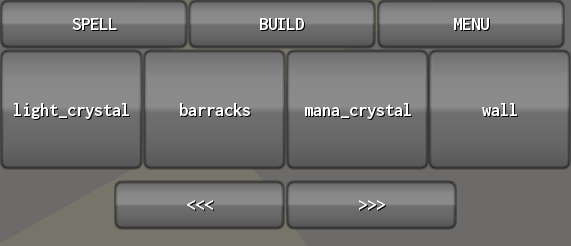
\includegraphics[width=\textwidth]{../img/tool-build.png}
    \caption{Window that allows the player to place buildings.}
    \label{gui-build}
\end{figure}

Most of the buildings can be unlocked through the research window.\footnote{Those that are not are available to the player from the start of
the game.} Similarly to spells, a research node \emph{BUILDING NAME} unlocks a
building called \emph{building\_name}. The next list contains all of the buildings our players can build, along with their price
in gold noted next to their names in parentheses and their description.

\begin{itemize}
    \item \emph{wall} (300) -- can be placed to separate rooms and to protect the dungeon.
    \item \emph{mine} (400) -- spawns a single ogre miner, which can mine walls and gold deposits.
    \item \emph{slow\_trap} (400) -- halves the speed of enemies that step on it for five seconds with a cooldown period
        \footnote{By \emph{cooldown period} we refer to the amount of time between two applications of the trap's effects.}
        of thirty seconds.
    \item \emph{mana\_crystal} (500) -- increases maximum mana and mana regeneration of the player.
    \item \emph{gold\_vault} (500) -- used to store gold.
    \item \emph{light\_crystal} (500) -- used as a source of light.
    \item \emph{fortified\_wall} (600) -- a strong wall that can be used to protect the dungeon.
    \item \emph{teleport\_trap} (600) -- teleports enemies that step on it to a random spot on the map with a cooldown period
        of thirty seconds.
    \item \emph{damage\_trap} (600) -- damages enemies that step on it with a cooldown period of thirty seconds.
    \item \emph{kill\_trap} (600) -- kills enemies that step on it with a cooldown period of thirty seconds.
    \item \emph{freeze\_trap} (800) -- freezes enemies that step on it in place for fice seconds with a cooldown period of thirty seconds.
    \item \emph{barracks} (1000) -- spawns a single ogre warrior, which is a melee combat minion.
    \item \emph{ice\_tower} (1500) -- spawns a single ogre ice mage, which is a ranged combat minion that can cast freezing waves.
    \item \emph{light\_mana\_crystal} (1500) -- used as a source of light which increases maximum mana and mana regeneration of the
        player.
    \item \emph{thunder\_tower} (1750) -- spawns a single ogre thunder mage, which is a ranged combat minion that can cast lightning bolts.
    \item \emph{fire\_tower} (1800) -- spawns a single ogre fire mage, which is a ranged combat minion that can cast meteors.
    \item \emph{church} (2000) -- spawns a single ogre cleric, which is a range combat minion that can heal others.
    \item \emph{chaos\_tower} (5000) -- spawns a single ogre chaos mage, which is a ranged combat minion that can cast random spells.
\end{itemize}

Beside these buildings, there is one additional building that the player cannot build, but is built by the game whenever a new level is
generated -- the dungeon throne.

\section{Options menu}

If we look at the options menu window, which can be accessed from either the main menu or the ingame menu bar, we will be presented with a
few basic options, which can be seen in Figure~\ref{gui-options}. These
options include the ability to change the resolution and fullscreen status of the game. Both of these options are controlled by a list
with predefined choices which can be clicked on to change the values that are located below the lists.
Once we choose new values for these options, we can apply them by clicking on the \emph{APPLY} button.

Below these graphical options, we can see pairs of buttons and labels. Each of these labels represents an action in the game and its
corresponding button the key that is assigned to action. To change the key binding, we can click on the button with our left mouse button
and then press a new key, which will be newly bound to the action. Note that this key binding change is only temporary and the key bindings
will reset when we restart the game. To save our new key bindings, we can use the \emph{APPLY} button, which will ensure that these new
key bindings will persist between games.

The \emph{SPELL/BUILD 1-4} actions correspond to the four buttons used to cast spells and buildings and their effect depends on the
currently selected tool bar. \emph{NEXT SPELL/BUILD} and \emph{PREV SPELL/BUILD} move the spell or building selection to the right and
to the left, respectively.

The \emph{SPELL TAB}, \emph{BUILD TAB} and \emph{MENU TAB} actions change the current tool bar between the spell selection, building
selection and mini menu. \emph{RESET CAMERA} returns the game's view back to the center of the map. Lastly, \emph{QUICK SAVE} and
\emph{QUICK LOAD} are used for fast and simple saving or loading of the save file \texttt{saves/quick\_save.lua}.

\begin{figure}[H]
    \centering
    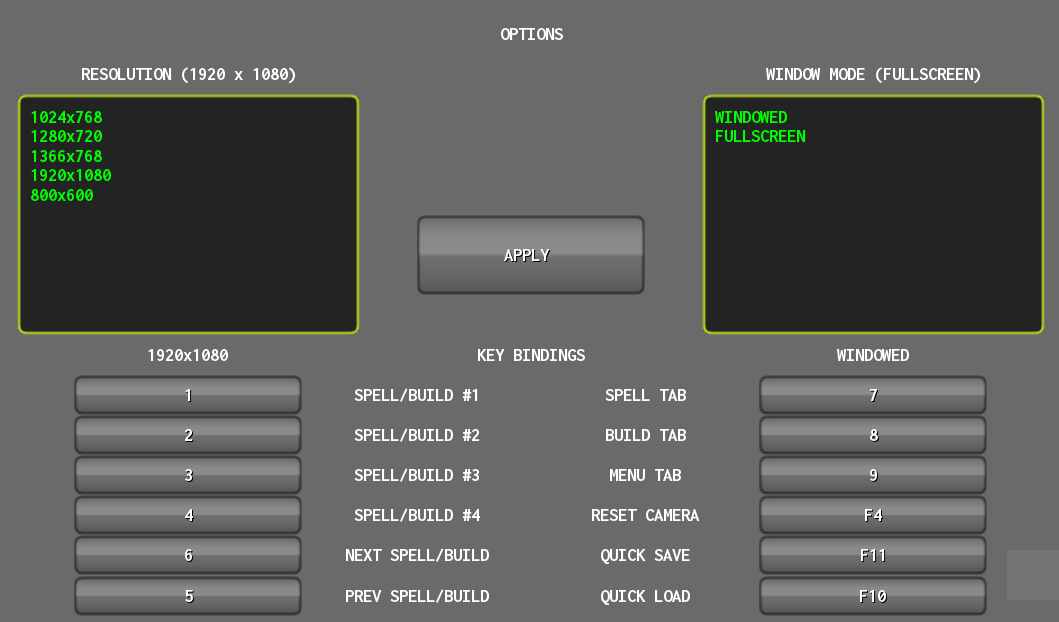
\includegraphics[width=\textwidth]{../img/gui-options.png}
    \caption{Options menu which contains basic graphics options and key binding.}
    \label{gui-options}
\end{figure}

Besides these rebindable actions, the game contains three actions that are used mainly for mod prototyping and testing and cannot be rebound.
If we press the \emph{Grave} key\footnote{On starndard english, american and czech keyboards, this key is generally located above the
\emph{TAB} key and below the \emph{ESC} key and is used to input a semicolon or a tilde.} we will bring up the game's development console,
which accepts Lua code and can interpret this code with the \emph{EXECUTE} button. If we hold the \emph{Shift} key pressed while we click
on the \emph{Grave} key, we bring up the entity creator window that lets us to place all entities in the game without any cost. Lastly,
the \emph{0} key on the numeric pad toggles between fixed camera mode and free camera mode.
